\documentclass{article}
\usepackage{graphicx}
\graphicspath{ {../Results/} }

\begin{document}

\title{HPC Practical{}}
\author{Jacob Griffiths}

\maketitle

\section{Neutral Theory}

\subsection{Question 8}
Despite no species having superior fitness in a neutral model, 
the system will always converge to monodominance
as time elapses. This is because as a species becomes more
numerous by chance, they now have a higher probability of 
being selected by the model to replace the removed individual at
the next neutral step. This advantage will perpetuate until only 
one species remains.

\begin{figure}[!htb]
    \center{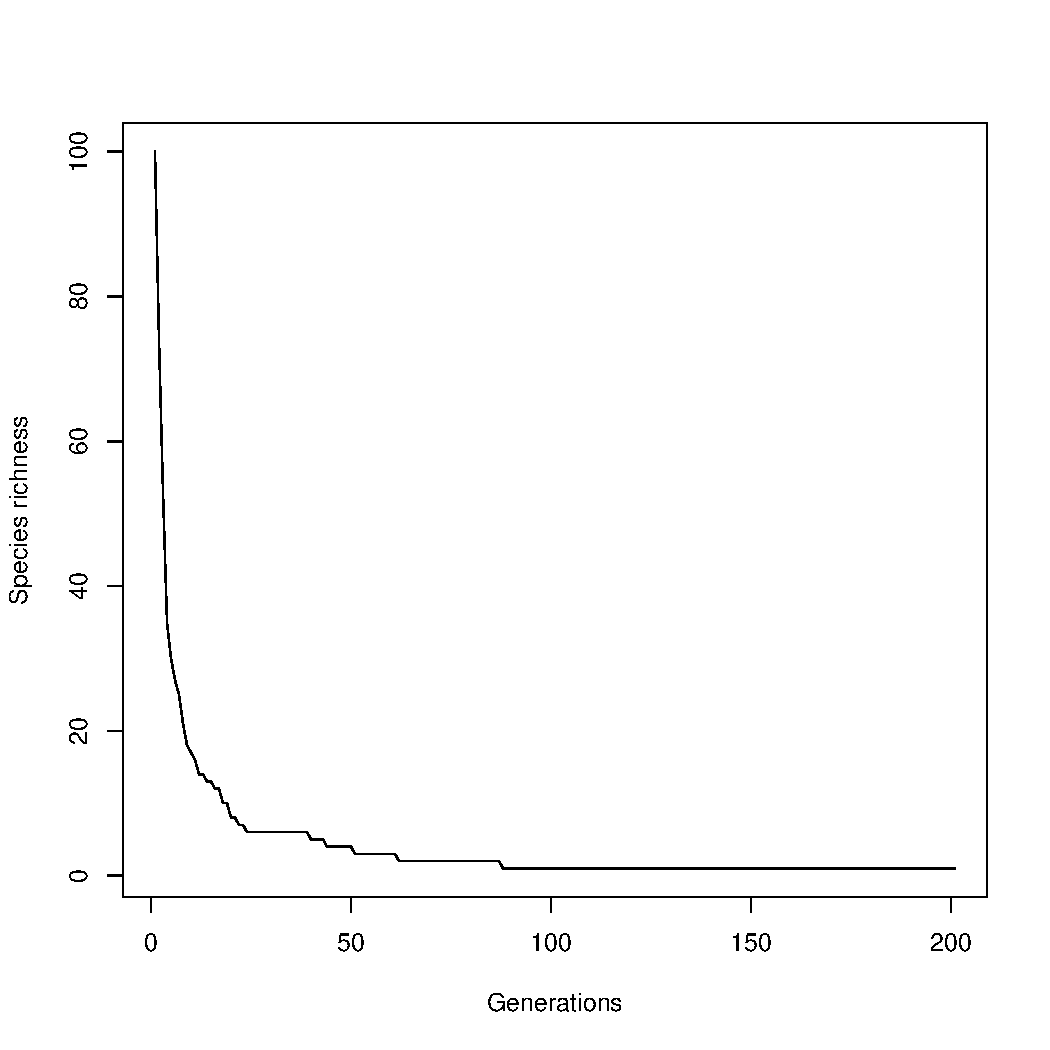
\includegraphics[width=\textwidth]
    {../Results//question_8.pdf}}
    \caption{\label{fig:my-label} figure text here}
  \end{figure}



\end{document}